\section{Applications and evidence map}
\label{sec:applications}

TableÂ~\ref{tab:T6-evidence-map} lists the papers and information on
model class, integration role, training design and validation. To align
the narrative synthesis with the quantitative figures, the applications
are grouped into five application-target domains: integrated and
distributed multi-energy systems; system design and expansion; thermal
and building energy systems; power-system operation and markets; and
power flow, network security and grid planning. The former detailed
application groups are retained below as subgroups within these five
domains.

\begin{figure*}[!t]
\centering
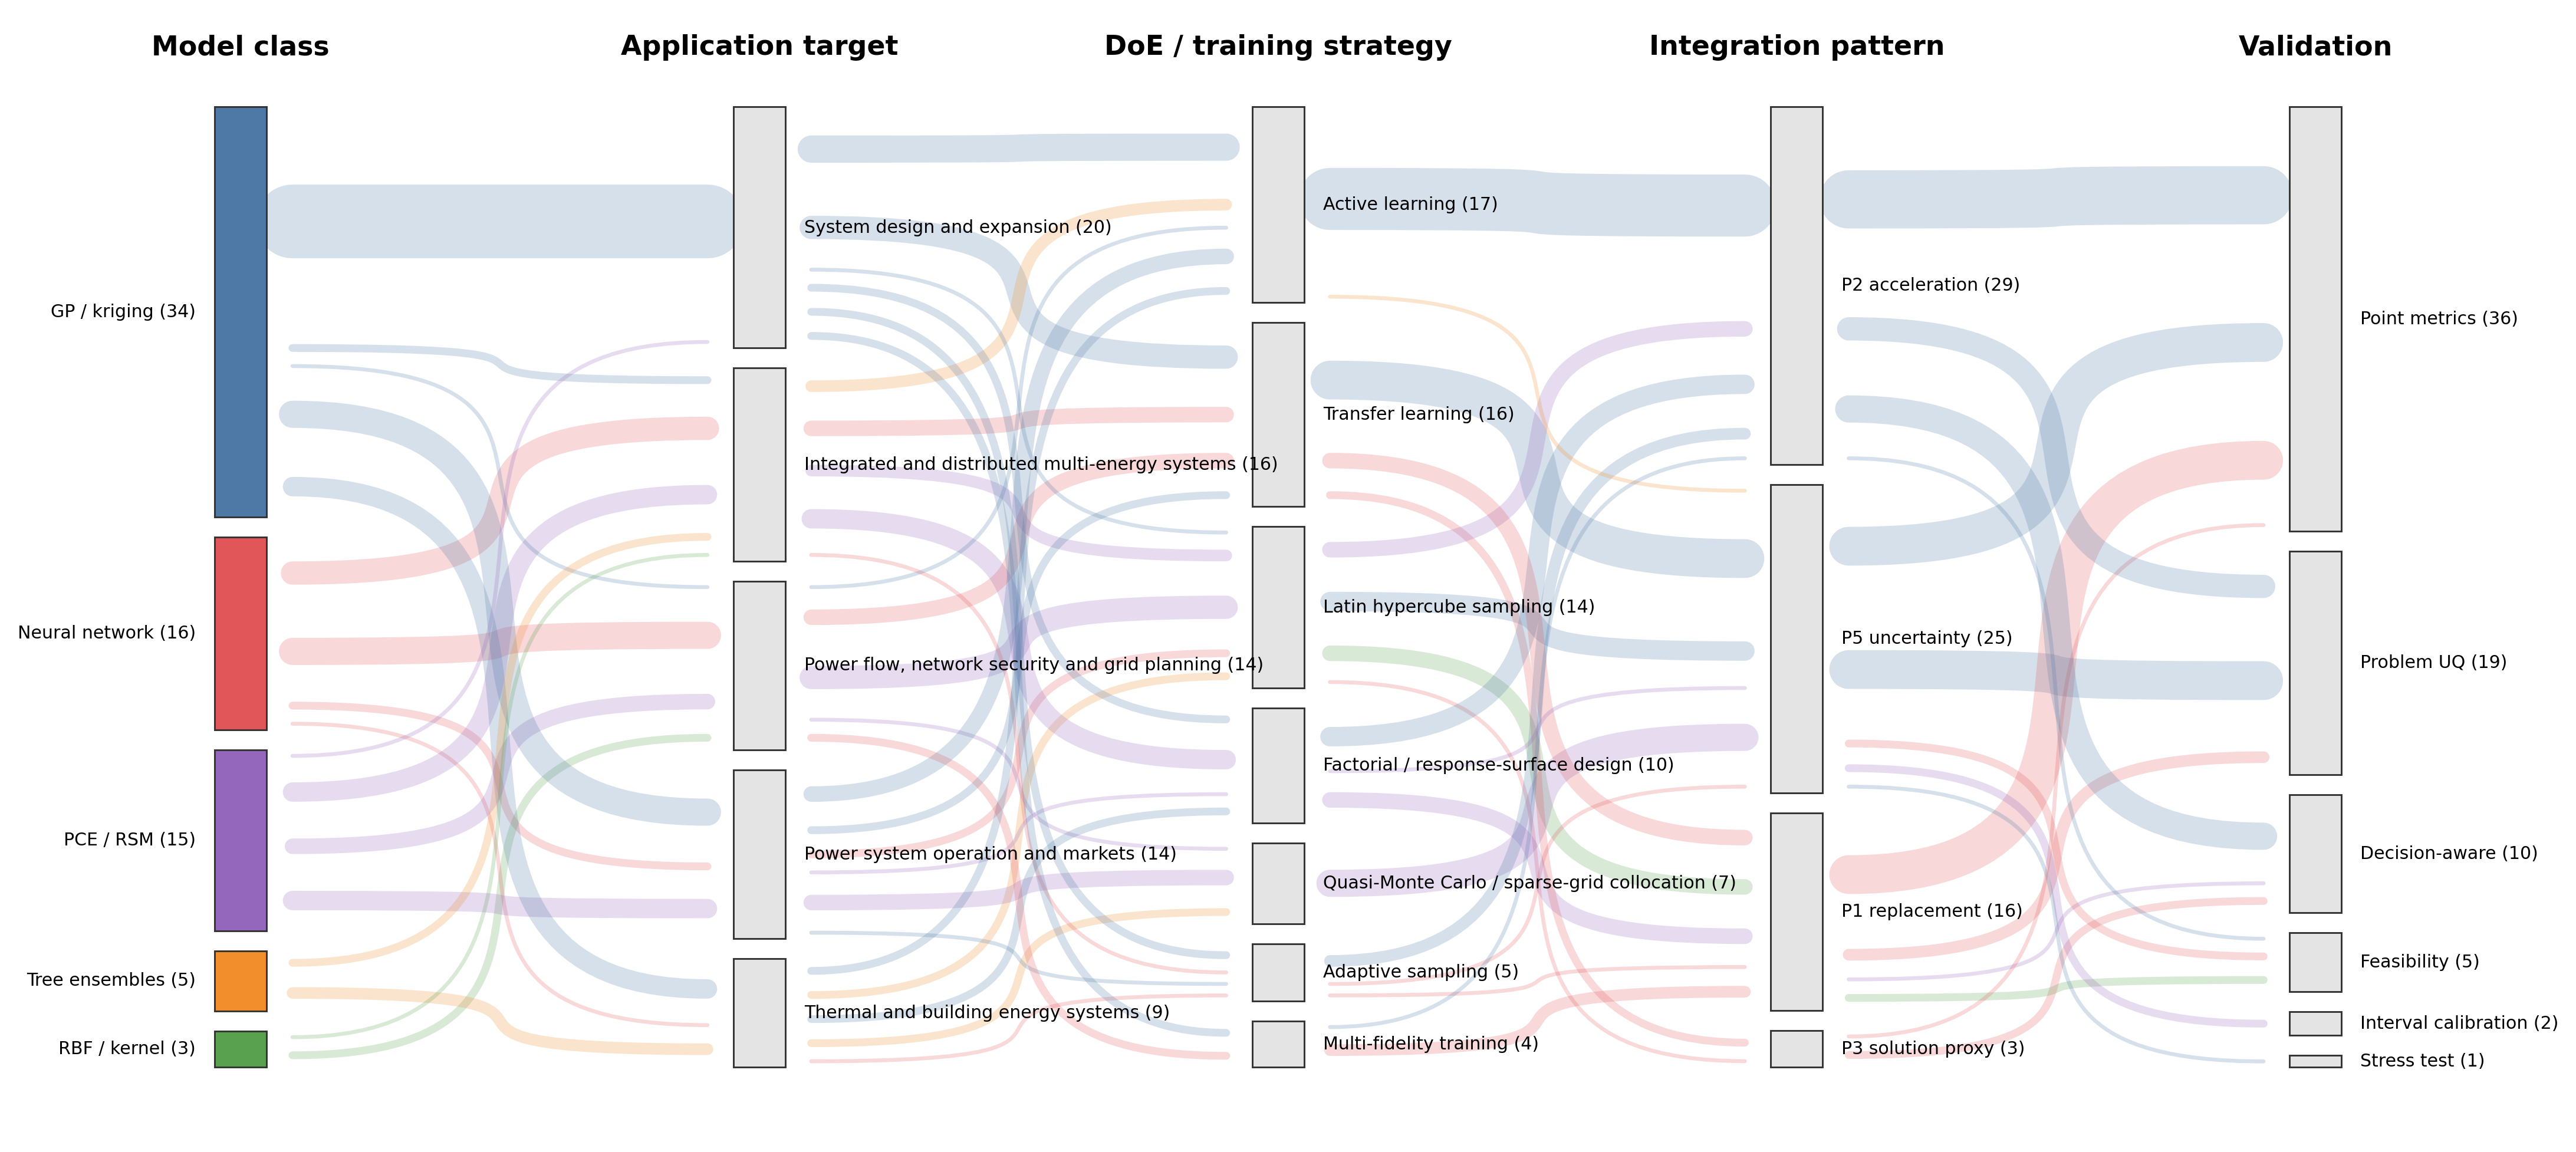
\includegraphics[width=\textwidth]{../figures/fig_taxonomy_alluvial_flow_evidence.png}
\caption{Evidence-based flow from surrogate model class through DoE and training, integration pattern and validation practice. Only studies with explicit assignments across the plotted stages are included.}
\label{fig:evidence-alluvial}
\end{figure*}

FigureÂ~\ref{fig:evidence-alluvial} shows how the methodological
dimensions are connected across the evidence base. FigureÂ~\ref{fig:application-target-taxonomy} then compares model
classes, DoE and training choices, integration patterns and validation
practices across the same five application-target domains. Counts in
the panels refer to explicit study-level category assignments; one study
can contribute to more than one DoE or validation category.

\begin{figure*}[!t]
\centering
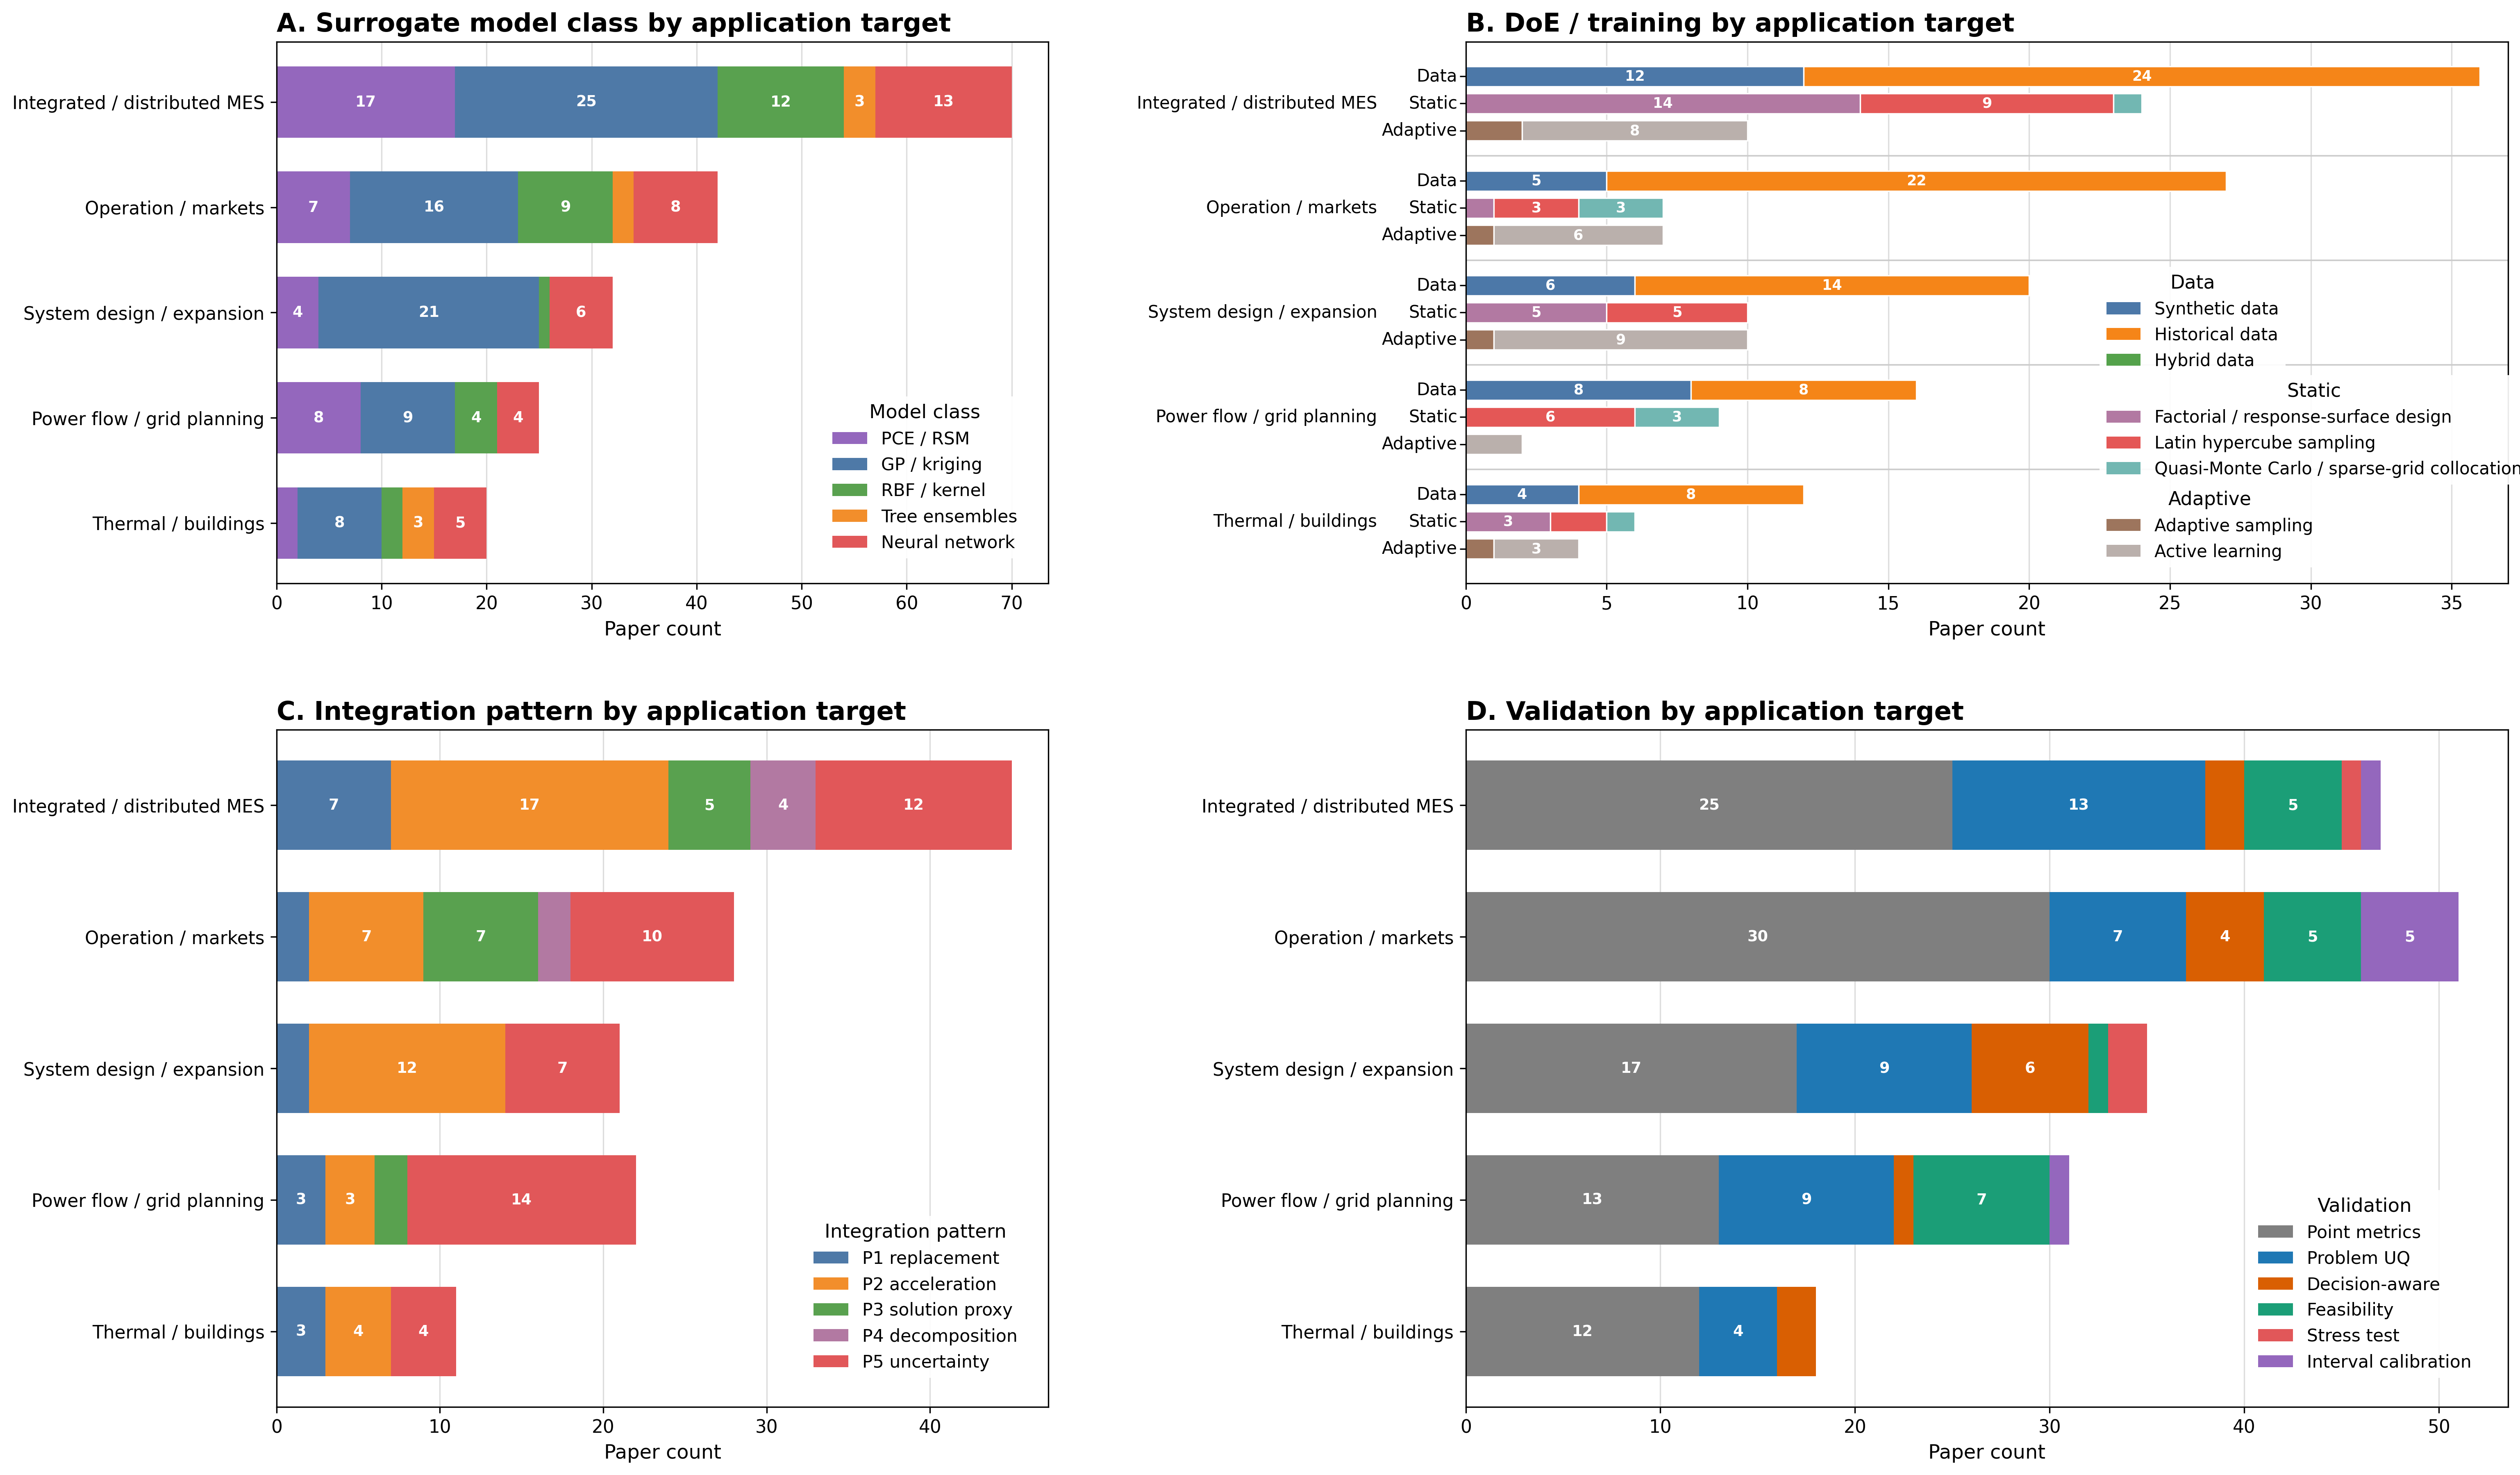
\includegraphics[width=\textwidth]{../figures/fig_four_panel_application_target_taxonomy.png}
\caption{Quantitative evidence by application target. Panels A to D show the surrogate model class, data source and DoE strategy, integration pattern, and validation practice. Counts are based on explicit study-level assignments; unresolved labels are omitted.}
\label{fig:application-target-taxonomy}
\end{figure*}

\subsubsection{Integrated and distributed multi-energy systems: multi-energy and sector-coupled systems}
\label{sec:apps:mes}

MES applications cover electricity--heat--gas coupling, integrated
dispatch and system design. Several studies use surrogates as P1
replacements for repeated inner optimisation solves. Ren et
al.Â~\cite{Ren2024} use a NN-based surrogate for heterogeneous multi-energy
storage deployment and place the training inputs by LHS. Jalving et
al.Â~\cite{Jalving2023} use a NN-based surrogate in conceptual design and
optimisation of integrated energy systems, and Franzoso et
al.Â~\cite{Franzoso2025} use a NN-based surrogate-assisted formulation in the
context of DRL for energy-system analysis and optimisation.

A second group focuses on uncertainty-aware MES operation. Zhou et
al.Â~\cite{Zhou20181} use a GP/kriging surrogate in robust optimisation of an
integrated community energy system and report prediction-interval
calibration. Dong et al.Â~\cite{Dong2022} also use a GP/kriging surrogate for
uncertainty propagation in robust MPC of an RES-CCHP system. Wang et
al.Â~\cite{Wang2020202933} use a PCE/RSM surrogate to replace repeated inner
solves in IES scheduling with scheduling elasticity. Dong et
al.Â~\cite{Dong2023} use a PCE/RSM surrogate for chance-constrained IES
dispatch, with sparse-grid or PCE-collocation sampling and feasibility
or constraint-violation checks. Zheng et al.Â~\cite{Zheng20231907} use a
GP/kriging surrogate for distributed electricity--heat dispatch with
variable mass flow and report feasibility or constraint-violation
validation. Shi et al.Â~\cite{Shi2024__2} use a GP/kriging surrogate in a
decomposition-layer setting for regional IES load forecasting.

\subsubsection{System design and expansion: multi-objective energy system design}
\label{sec:apps:moo}

MOO energy-system design is mainly a P2 application area, because many
candidate designs must be evaluated while approximating a Pareto front.
PCE/RSM surrogates are used inside outer MOO or evolutionary search in
campus multi-energy systems \cite{Dong2024}, solar-integrated trigeneration
systems with structured DoE \cite{Salahinezhad2025}, strategic stochastic
planning with feasibility or constraint-violation validation
\cite{alahmad_enhancing_2025}, and stochastic optimisation of renewable and
green technologies with stress-test validation
\cite{alahmad_optimizing_2025}. The same PCE/RSM pattern is used for
hydrogen systems and demand response with RES and EVs
\cite{ali_optimizing_2025}, shared BESS placement with feasibility or
constraint-violation validation \cite{an_multi-objective_2025}, renewable
planning with an improved Frilled Lizard algorithm
\cite{bendriss_novel_2025}, biomass--solar--wind multi-energy systems with
feasibility or constraint-violation validation
\cite{chen_multi-objective_2025-1}, NSGA-II-based MOO
\cite{cortes-caicedo_multi-objective_2025}, pumped-storage operation
\cite{liang_high_2024}, Power-to-X conversion \cite{malla_sg_optimization_2024},
and green-hydrogen HRES design with factorial training designs
\cite{tezer_multi-objective_2025}.

NN-based surrogates are also used in outer MOO or evolutionary search.
Wang et al.Â~\cite{Wang2024} use a NN surrogate for PV-based hydrogen--oxygen
co-production and report feasibility or constraint-violation validation.
Lalitha et al.Â~\cite{Lalitha20231401} use a NN surrogate in
surrogate-assisted particle swarm optimisation for microgrid protection.
Reis et al.Â~\cite{Reis2025} use a NN surrogate in symmetry-guided
surrogate-assisted NSGA-II, with further simulations selected by
BO-style active learning. Bagheri et al.Â~\cite{bagheri_miqcp-based_2025} use
a NN surrogate in an MIQCP-based MOO operation strategy for
renewables-integrated smart systems. Tian et al.Â~\cite{tian_building_2025}
use a NN surrogate trained from historically observed operating data for
building design and operation MOO and report feasibility or
constraint-violation validation.

Other MOO studies use GP/kriging or RBF-type surrogates. Zhang et
al.Â~\cite{Zhang20234075} use a GP/kriging surrogate for multimodal MOO of an
HRES. Han et al.Â~\cite{Han2018622} use an RBF/kernel surrogate for dynamic
VAR planning with short-term voltage considerations. Not all MOO-related
studies are pure outer-loop search cases: Dong et al.Â~\cite{Dong2023__2} use
a PCE/RSM surrogate to replace inner optimisation solves in robust IES
scheduling, while Abbas et al.Â~\cite{abbas_optimal_2024} use a PCE/RSM
surrogate in a decomposition-layer setting for grid-connected
distributed-resource scheduling and report feasibility or
constraint-violation validation.

\subsubsection{Integrated and distributed multi-energy systems: microgrids and energy hubs}
\label{sec:apps:microgrid}

Microgrid, energy-hub and VPP studies cover controller tuning,
scheduling, sizing, bidding and energy management. Several
controller-tuning papers use PCE/RSM surrogates inside outer MOO or
evolutionary search. Hussien et al.Â~\cite{Hussien20211883} use factorial
designs for PI-control tuning with a sunflower optimisation algorithm.
Hussien et al.Â~\cite{Hussien20226442}, Hussien et al.Â~\cite{Hussien202190577}
and Hussien et al.Â~\cite{Hussien202415075} use discrete-factor
response-surface fitting for PI-control tuning in autonomous or islanded
microgrid operation. Arar Tahir et al.Â~\cite{arar_tahir_scientific_2023} use
LHS for a PCE/RSM surrogate in optimisation of microgrids with renewable
energy systems. Batista et al.Â~\cite{batista_optimizing_2023} use the same
surrogate role for HRES-powered reverse-osmosis plants.

RBF/kernel surrogates are mainly used as P1 replacements for repeated
evaluations in microgrid and energy-hub operation. Faraji et
al.Â~\cite{Faraji2020157284} use an RBF/kernel surrogate for day-ahead
self-scheduling and operation of prosumer microgrids. Wang et
al.Â~\cite{Wang20192635} use an RBF/kernel surrogate trained from
historically observed operating data for power-management optimisation
in a hybrid microgrid. Lu et al.Â~\cite{Lu20232989} use an RBF/kernel
surrogate trained from historical operating data for distributed online
microgrid dispatch and report feasibility or constraint-violation
validation. Wu et al.Â~\cite{Wu2021} use an RBF/kernel surrogate for AA-CAES
energy-hub bidding and scheduling, with further simulations selected by
BO. Zhang et al.Â~\cite{Zhang20203731} use an RBF/kernel surrogate for
two-stage isolated-microgrid operation and transfer information across
related datasets.

GP/kriging and NN surrogates are also common P1 replacements in this
application group. Eseye et al.Â~\cite{Eseye201991463} use a GP/kriging
surrogate for electricity-demand modelling with integrated feature
selection. Rigo-Mariani et al.Â~\cite{Rigo-Mariani20171762} use a GP/kriging
surrogate for integrated smart-microgrid design with storage. Gan et
al.Â~\cite{Gan2021695} use GP forecasting with MPC for an interconnected EMS,
and Kanwal et al.Â~\cite{Kanwal2018117} use SVM and GP regression for
PV-power modelling. Guo et al.Â~\cite{Guo20222057} use a NN surrogate for
optimal power allocation in islanded microgrids. Chaturvedi et
al.Â~\cite{Chaturvedi2024149} use a NN surrogate in RL-based integrated
control of DC microgrids. Roth et al.Â~\cite{Roth2019214} formulate a
modular MILP metamodel architecture for HRES design. Liu et
al.Â~\cite{Liu20242534} use a
hard-constrained NN surrogate for hybrid AC/DC microgrid energy
management.

Uncertainty-aware microgrid and VPP studies mainly follow P5.
Nematollahi et al.Â~\cite{Nematollahi2021} use a GP/kriging surrogate for DER
sizing and siting in active distribution networks. Kiani et
al.Â~\cite{Kiani20253021} use a GP/kriging surrogate for robust MPC in
islanded microgrid voltage control. Han et al.Â~\cite{Han2024} use a
GP/kriging surrogate for hierarchical robust day-ahead VPP--DSO
coordination. Pourmohammadi et al.Â~\cite{Pourmohammadi2023} use a PCE/RSM
surrogate for robust metamodel-based HRES design. Yang et
al.Â~\cite{Yang2024__2} use a PCE/RSM surrogate for robust day-ahead to
intra-day microgrid scheduling and include stress-test validation. Wang
et al.Â~\cite{Wang20211767} use an RBF/kernel surrogate for stochastic
residential demand response with UC and TOU pricing.

Other studies show additional integration roles within microgrid and
energy-hub applications. Kaewdornhan et al.Â~\cite{Kaewdornhan2022130373} use
a NN surrogate in outer MOO or evolutionary search for
distribution-network management with multi-microgrids and report
feasibility or constraint-violation validation. Perera et
al.Â~\cite{Perera2017187} use a NN surrogate for distributed energy-hub
design and select further simulations by active learning. Cao et
al.Â~\cite{Cao2023__2} replace inner solves in VPP co-optimisation with
electricity--heat--carbon trading and use LHS for the training inputs.
Xu et al.Â~\cite{Xu20184696} use a PCE/RSM surrogate to replace inner solves
in islanded-microgrid loadability analysis and represent uncertainty by
sparse-grid or PCE-collocation nodes. Li et al.Â~\cite{Li2023__3} train a
sparse variational GP surrogate on historical data to imitate
electricity and heat-flow calculations for multi-agent energy
management of multiple microgrids. Matta et
al.Â~\cite{Matta2026} use a GP/kriging surrogate with active learning for
near-optimal isolated-microgrid design and report prediction-interval
calibration. Velásquez et al.Â~\cite{velasquez_intelligence_2023} use an
RBF/kernel surrogate inside outer MOO or evolutionary search.

\subsubsection{Thermal and building energy systems: district heating and thermal storage}
\label{sec:apps:dh}

DH and thermal-storage studies are closely related to the modelling
setting discussed earlier, because building or thermal-network models
are often too expensive to embed directly in system-level optimisation.
Hirvonen et al.Â~\cite{Hirvonen2017323} use a NN metamodel in MOO of a
high-latitude solar community and report feasibility or
constraint-violation validation. Sánchez-Zabala et
al.Â~\cite{Sánchez-Zabala2024} compare several machine-learning algorithms
and use boosting-based building metamodels in a district
energy-management optimisation testbed. They report point-prediction
accuracy and validate the models on buildings not used for training.

Further DH-related studies use surrogates either as P1 replacements or
as P5 uncertainty components. Weinberger et al.Â~\cite{Weinberger2018555} use
a NN surrogate for combined heat and power analysis and train it with a
Box--Behnken design. Reich et al.Â~\cite{Reich2020} use a GP/kriging
surrogate for predictive DH control. Chaudhry et al.Â~\cite{Chaudhry2024} use
a PCE/RSM surrogate for robust fifth-generation DHC analysis, with
sparse-grid or PCE-collocation nodes for uncertain inputs. Du et
al.Â~\cite{Du2025} use a NN surrogate to improve energy flexibility of an
integrated system under uncertainty.

\subsubsection{Power-system operation and markets: economic dispatch and unit commitment}
\label{sec:apps:dispatch}

Dispatch and UC studies focus on repeated LP/MILP-type solves, nonconvex
economic dispatch, stochastic dispatch and learning-based proxies. NN
surrogates are often used as P1 replacements for SCUC, SCED and
economic-dispatch evaluations. Wu et al.Â~\cite{Wu2022231} use a NN surrogate
for SCUC with uncertain wind power. Chen et al.Â~\cite{Chen20244723} use a NN
surrogate as an end-to-end feasible optimisation proxy for large-scale
economic dispatch and report regret or optimality-gap checks. Chen et
al.Â~\cite{Chen2022} use a NN surrogate for large-scale SCED and report
feasibility or constraint-violation validation. Xu et al.Â~\cite{Xu20223066}
use an ensemble DNN for nonconvex economic dispatch, and Guo et
al.Â~\cite{Guo202115024} use a learning-based approach for economic dispatch
in smart grids.

PCE/RSM surrogates are mainly used for uncertainty propagation in
stochastic or reliability-constrained dispatch. Safta et
al.Â~\cite{Safta20172535} use PCE/RSM for stochastic economic dispatch,
represent uncertain inputs by sparse-grid or PCE-collocation nodes and
report feasibility or constraint-violation validation. Wang et
al.Â~\cite{Wang2022812}, Li et al.Â~\cite{Li20191438} and Lu et al.Â~\cite{Lu201991827}
also use PCE/RSM with sparse-grid or PCE-collocation nodes for
stochastic economic dispatch under renewable uncertainty. Pan et
al.Â~\cite{Pan20244422} use PCE/RSM for reliability-constrained economic
dispatch, also with sparse-grid or PCE-collocation nodes and feasibility
or constraint-violation validation.

Other dispatch applications use RBF/kernel, PCE/RSM or GP/kriging
surrogates as P1 replacements. Rafi et al.Â~\cite{Rafi202132436} use an
RBF/kernel surrogate in short-term load forecasting with integrated CNN
and LSTM components. Dullinger et al.Â~\cite{Dullinger20181646} use an
RBF/kernel surrogate for MILP-based HVAC predictive control. Goudarzi et
al.Â~\cite{Goudarzi2017667} use an RBF/kernel surrogate for real-time
scheduling of generating units. Ahmad et al.Â~\cite{Ahmad202451} use a
PCE/RSM surrogate for wastewater electrolysis and train it with a
Box--Behnken design. Rixhon et al.Â~\cite{Rixhon2021} use a PCE/RSM surrogate
for electrofuels in the Belgian energy transition, with quasi-Monte
Carlo sampling. Angizeh et al.Â~\cite{Angizeh2023134995} use a GP/kriging
surrogate for grid integration of storage and renewables and report
prediction-interval calibration. Yan et al.Â~\cite{Yan2019625} use a
GP/kriging surrogate for wind-generation interval forecasts and also
report prediction-interval calibration.

GP/kriging also appears in search and uncertainty settings. Nikolaidis
et al.Â~\cite{Nikolaidis2021} use GP-based BO for data-driven UC, where
further simulations are chosen by acquisition-driven active learning.
Lin et al.Â~\cite{Lin2023} use a GP/kriging surrogate in a search-loop
formulation for combined economic/emission dispatch. Hu et
al.Â~\cite{Hu2021671} use GP/kriging for uncertainty propagation in
stochastic economic dispatch, with sparse-grid or PCE-collocation nodes.
Hu et al.Â~\cite{Hu2020} use GP emulation for stochastic economic dispatch
and place training inputs by LHS. Further dispatch and UC examples
include deep neural networks embedded in Surrogate Lagrangian
Relaxation for UC \cite{Wu2024391}, a NN surrogate inside an
adaptive bat algorithm for large-scale economic dispatch \cite{Pang2023},
and a constraint-aware neural surrogate for joint chance-constrained UC
\cite{Liang20246508}.

\subsubsection{Power flow, network security and grid planning: optimal power flow and AC relaxations}
\label{sec:apps:opf}

OPF work mainly uses surrogates to approximate nonlinear AC-OPF or
load-flow evaluations, or to propagate uncertainty in chance-constrained
and robust formulations. PCE/RSM surrogates are used for
chance-constrained AC-OPF by Muhlpfordt et al.Â~\cite{Muhlpfordt20194806}, PV
hosting-capacity calculation by Koirala et al.Â~\cite{Koirala20242284}, OPF
with non-Gaussian uncertainties by Muhlpfordt et
al.Â~\cite{Muhlpfordt20174490}, iterative response-surface chance-constrained
AC-OPF by Xu et al.Â~\cite{Xu20212696}, and current--voltage OPF by Van Acker
et al.Â~\cite{Van Acker2022}. These PCE/RSM studies use sparse-grid or
PCE-collocation nodes for uncertain inputs, and Xu et al.Â~\cite{Xu20212696}
and Van Acker et al.Â~\cite{Van Acker2022} report feasibility or
constraint-violation validation.

RBF/kernel surrogates are used as P1 replacements in reliability,
stability, prediction and TCSC-allocation problems. Urgun et
al.Â~\cite{Urgun20202791} use an RBF/kernel surrogate for
composite-power-system reliability and place training inputs by LHS. Liu
et al.Â~\cite{Liu20223726} use an RBF/kernel surrogate for
small-signal-stability-constrained OPF. Wu et al.Â~\cite{Wu2021__2} use an
RBF/kernel surrogate for short-term power prediction with an improved
bird swarm algorithm. Mahapatra et al.Â~\cite{Mahapatra20161921} and
Mahapatra et al.Â~\cite{Mahapatra2022721} use RBF/kernel surrogates for TCSC
location, sizing or allocation in OPF-related settings.

GP/kriging surrogates are used both for OPF replacement and
chance-constrained OPF. Deng et al.Â~\cite{Deng2020831} use kriging-assisted
surrogate evolutionary computation for OPF and add training points
sequentially by infill rules. Mitrovic et al.Â~\cite{Mitrovic2023__2} use
hybrid sparse GPs for data-driven chance-constrained AC-OPF and report
feasibility or constraint-violation validation. Mitrovic et
al.Â~\cite{Mitrovic2023__3} use GP-based chance-constrained OPF in a
software-tool setting. Katkar et al.Â~\cite{Katkar2025} use GP/kriging in an
ensemble surrogate archive-assisted metaheuristic for OPF-related
multi-modal optimisation.

Distribution-network planning and stochastic OPF studies also use
uncertainty-focused surrogates. Fu et al.Â~\cite{Fu20202904} use PCE/RSM for
stochastic distribution-network planning and train with LHS. Fu et
al.Â~\cite{Fu2022} use PCE/RSM for capacitor planning under PV uncertainty,
with discrete-factor response-surface fitting and feasibility or
constraint-violation validation. Engelmann et al.Â~\cite{Engelmann20186188}
use PCE/RSM for distributed stochastic AC-OPF, with sparse-grid or
PCE-collocation nodes and feasibility or constraint-violation
validation. Zhang et al.Â~\cite{Zhang2024821} use GP/kriging for
distributionally robust chance-constrained conservation voltage
reduction, and Liu et al.Â~\cite{Liu20222679} use GP/kriging for data-driven
probabilistic load-flow studies.

NN, constraint-aware NN and tree-ensemble surrogates appear in fast
control and OPF proxy formulations. Su et al.Â~\cite{Su2022315} use a NN
surrogate for fast preventive control and place training inputs by LHS.
Li et al.Â~\cite{Li202359995} use a NN surrogate for optimisation with hard
linear constraints, transfer information across related datasets and
report feasibility or constraint-violation validation. Chen et
al.Â~\cite{Chen2023657} use a constraint-aware neural surrogate for joint
chance-constrained OPF and report feasibility or constraint-violation
validation. Lei et al.Â~\cite{Lei20247417} use a constraint-aware neural
surrogate for chance-constrained DC-OPF with affine control policy and
report feasibility or constraint-violation validation. Srithapon et
al.Â~\cite{Srithapon202134395} use a NN surrogate inside outer MOO or
evolutionary search for probabilistic OPF in distribution networks. Li
et al.Â~\cite{Li2023__2} use neural networks with gauge mappings to
accelerate ADMM-based DC-OPF while enforcing local constraints.

\subsubsection{System design and expansion: capacity and generation expansion planning}
\label{sec:apps:expansion}

Expansion planning re-evaluates operational sub-models across investment
candidates. Park et al.Â~\cite{Park2019} use a NN surrogate in an outer
search-loop setting for physics-induced graph-neural-network wind-farm
power estimation. Jahangiri et al.Â~\cite{Jahangiri20244849} use a NN
surrogate for Canadian provincial power-system decarbonisation analysis,
and Jahangiri et al.Â~\cite{Jahangiri2023} use a NN surrogate-assisted
formulation to explore the Canadian decarbonisation design space.

Uncertainty-aware expansion studies mainly use GP/kriging. Kim et
al.Â~\cite{Kim2021} use a GP/kriging surrogate for probabilistic
wind-energy-potential modelling in power-grid expansion planning. Lawson
et al.Â~\cite{Lawson201647} use a GP/kriging surrogate in a Bayesian
framework for power-network planning under uncertainty. Volodina et
al.Â~\cite{Volodina2022} use a GP/kriging surrogate for uncertainty
propagation in a network of energy models, with LHS training inputs and
prediction-interval calibration.

Other expansion-planning examples use different model classes and roles.
Rodgers et al.Â~\cite{Rodgers2018951} use a PCE/RSM surrogate inside outer
MOO or evolutionary search for generation expansion planning with health
and societal damages. Pérez-Uresti et al.Â~\cite{Pérez-Uresti2023} use a NN
surrogate to replace expensive inner optimisation solves in strategic
hydrogen-economy investment planning. Yang et al.Â~\cite{Yang2025} use a
tree-ensemble surrogate inside adaptive multi-objective BO for
interconnected capacity planning, with further simulations selected by
acquisition-driven active learning.

\subsection{Synthesis: where surrogates help, where they do not}
\label{sec:apps:synthesis}

Taken together, the evidence map supports four observations. *First*,
the five domains differ more clearly by integration role than by model
class. Panel A of
FigureÂ~\ref{fig:application-target-taxonomy} shows GP/kriging as the
largest model-class category in every domain, although PCE/RSM,
RBF/kernel and neural models remain substantial in specific
applications. *Second*, Panel C shows that P2 acceleration is the
largest integration category in integrated and distributed MES. P5
uncertainty is largest in system design and expansion, power flow and
grid planning, and power-system operation and markets. Thermal and
building applications are split more evenly between P1 replacement, P2
acceleration and P5 uncertainty. These
domain-level patterns are consistent with the cross-dimensional flows
in FigureÂ~\ref{fig:evidence-alluvial}. *Third*, Panel B shows that
historical data form the largest recorded data-source category in all
five domains, although in power flow and grid planning the historical
count is tied with Latin-hypercube sampling when data-source and DoE
categories are viewed together.
*Fourth*, Panel D confirms that point metrics dominate validation in all
five domains. Problem-level uncertainty is the next most frequent
category, while feasibility, stress testing, interval calibration and
decision-aware evaluation remain less common. For integrated MES and
system-design applications, an open issue therefore remains how
surrogate-derived Pareto or robust solutions should be validated and
communicated to decision makers
\cite{Mylonopoulos202332697,Lim2025}.
